\documentclass[aspectratio=169,11pt]{beamer}
\usetheme{Madrid}
\usecolortheme{default}
\usepackage{amsmath,amssymb,booktabs,tikz}
\usepackage[style=authoryear, backend=biber]{biblatex}
\addbibresource{ref.bib}
\usetikzlibrary{arrows.meta,positioning}
\title[Deep DR Estimation]{Deep Neural Networks for Doubly Robust Estimation\\with Nonprobability Survey Samples}
\author[Yuqing He]{Yuqing He \\ \small Based on : Dai, Luo, Lou, Wang \& Lu (2026)}
\date{June 9, 2026}
\begin{document}
\begin{frame}
  \titlepage
\end{frame}
\begin{frame}{Motivation: integrating two imperfect data sources}
\begin{columns}[T]
\column{0.52\textwidth}
\begin{itemize}
  \item \textbf{Nonprobability sample} $S_A$: rich outcome $y$, but unknown selection mechanism.
  \item \textbf{Probability sample} $S_B$: design weights and representative covariates $x$, but often no $y$.
  \item Goal: estimate the finite-population mean
  \[
    \mu_y=\frac{1}{N}\sum_{i=1}^N y_i.
  \]
\end{itemize}
\column{0.48\textwidth}
\centering
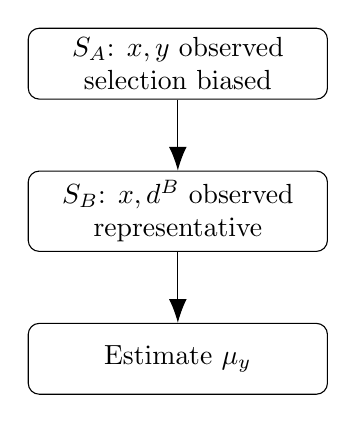
\begin{tikzpicture}[node distance=0.9cm, every node/.style={align=center}]
  \node[draw, rounded corners, minimum width=3.8cm, minimum height=0.9cm] (A) {$S_A$: $x,y$ observed\\selection biased};
  \node[draw, rounded corners, below=of A, minimum width=3.8cm, minimum height=0.9cm] (B) {$S_B$: $x,d^B$ observed\\representative};
  \node[draw, rounded corners, below=of B, minimum width=3.8cm, minimum height=0.9cm] (M) {Estimate $\mu_y$};
  \draw[-{Latex[length=3mm]}] (A) -- (B);
  \draw[-{Latex[length=3mm]}] (B) -- (M);
\end{tikzpicture}
\end{columns}
\end{frame}

\begin{frame}{Formal setup and notation}
\begin{itemize}
  \item Finite population $U=\{1,\ldots,N\}$; target parameter:
  $\mu_y=\frac{1}{N}\sum_{i=1}^N y_i.$
  \item \textbf{Nonprobability sample} $S_A$, size $n_A$: observe $(x_i,y_i)$. Selection indicator $R_i=I(i\in S_A)$, with $\pi_i^A=P_q(R_i=1\mid x_i,y_i)$.
  \item \textbf{Probability sample} $S_B$, size $n_B$: observe $(x_i,d_i^B)$, where $d_i^B=1/\pi_i^B$ and $\pi_i^B=P(i\in S_B)$ are the first-order inclusion probabilities.
  \item \textbf{Ignorability assumption}: $\pi_i^A=P(R_i=1\mid x_i)$ — selection depends only on observed $x$, not on $y$.
\end{itemize}
\begin{block}{Three classical strategies}
\begin{enumerate}
  \item Model the outcome: $m(x_i)=E(y_i\mid x_i)$ $\rightarrow$ predict $y$ for units in $S_B$.
  \item Model the selection: $\pi^A(x)=P(R=1\mid x)$ $\rightarrow$ inversely weight units in $S_A$.
  \item Combine both models (doubly robust).
\end{enumerate}
\end{block}
\end{frame}

\begin{frame}{Method 1: Regression / mass imputation (REG)}
\begin{block}{Procedure}
\begin{enumerate}
  \item Fit outcome model $m(x_i)=E(y_i\mid x_i)$ using $S_A$ (e.g., OLS).
  \item Predict $\hat{y}_i=m(x_i,\hat{\beta})$ for every unit in $S_B$.
  \item Estimate the population mean by
  \[
  \hat{\mu}_{REG}=\frac{1}{\hat{N}_B}\sum_{i\in S_B}d_i^B\,\hat{y}_i,\qquad
  \hat{N}_B=\sum_{i\in S_B}d_i^B.
  \]
\end{enumerate}
\end{block}
\vspace{0.2cm}
\begin{alertblock}{Critical assumption}
$m(x)$ is correctly specified. If $E(y\mid x)$ contains interactions, thresholds, or nonlinearities and a linear model is used, $\hat{\mu}_{REG}$ is inconsistent — no amount of design weighting can salvage a misspecified outcome model.
\end{alertblock}
\end{frame}

\begin{frame}{Method 2: Inverse probability weighting (IPW)}
\begin{block}{Procedure}
\begin{enumerate}
  \item Pool $S_A$ and $S_B$; define $R_i=I(i\in S_A)$.
  \item Fit propensity model $\pi^A(x)=P(R=1\mid x)$, typically logistic:
  $\operatorname{logit}[\pi^A(x)]=\alpha_0+x^{\top}\alpha.$
  \item Weight each unit in $S_A$ inversely to its selection probability:
  \[
  \hat{\mu}_{IPW}=\frac{1}{\hat{N}_A}\sum_{i\in S_A}\frac{1}{\hat{\pi}_i^A}y_i,\quad
  \hat{N}_A=\sum_{i\in S_A}\frac{1}{\hat{\pi}_i^A}.
  \]
\end{enumerate}
\end{block}
\vspace{0.1cm}
\begin{alertblock}{Critical assumption}
$\pi^A(x)$ follows the assumed parametric form (e.g., linear logit). If the true selection mechanism involves \textbf{nonlinearities, interactions, or unknown functional forms}, the logistic model is misspecified and IPW is inconsistent.
\end{alertblock}
\end{frame}

\begin{frame}{Method 3: Doubly robust (DR) estimation}
\begin{block}{Formula}
\[
\hat{\mu}_{DR}
=\frac{1}{\hat{N}_A}\sum_{i\in S_A}\frac{1}{\hat{\pi}_i^A}\{y_i-m(x_i,\hat{\beta})\}
+\frac{1}{\hat{N}_B}\sum_{i\in S_B}\frac{1}{\pi_i^B}\,m(x_i,\hat{\beta}).
\]
\end{block}
\vspace{0.05cm}
\begin{block}{Double robustness property}
$\hat{\mu}_{DR}$ is consistent if \textbf{either} the outcome model $m(x)$ \textbf{or} the propensity model $\pi^A(x)$ is correctly specified — not necessarily both. This is a genuine improvement over REG and IPW alone.
\end{block}
\vspace{0.1cm}
\begin{alertblock}{Remaining vulnerability}
When \textbf{both} working models are misspecified — e.g., the outcome regression is linear but $E(y\mid x)$ is nonlinear, \textit{and} the propensity is logistic but the true $\pi^A(x)$ is nonlinear — the DR estimator can also be inconsistent.\\
\textbf{Parametric double robustness $\neq$ nonparametric protection.}
\end{alertblock}
\end{frame}

\begin{frame}{Key idea of the paper}
The paper replaces the parametric propensity-score model by a DNN model:
\[
  \log\frac{\pi_i^A}{1-\pi_i^A}=g_0(x_i),
\]
where $g_0$ is an unknown nonparametric function.
\vspace{0.3cm}
\begin{center}
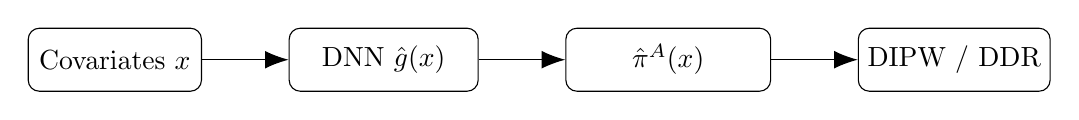
\begin{tikzpicture}[node distance=1.1cm]
  \node[draw, rounded corners, minimum width=2.2cm, minimum height=0.8cm] (x) {Covariates $x$};
  \node[draw, rounded corners, right=of x, minimum width=2.4cm, minimum height=0.8cm] (dnn) {DNN $\hat{g}(x)$};
  \node[draw, rounded corners, right=of dnn, minimum width=2.6cm, minimum height=0.8cm] (pi) {$\hat\pi^A(x)$};
  \node[draw, rounded corners, right=of pi, minimum width=2.4cm, minimum height=0.8cm] (est) {DIPW / DDR};
  \draw[-{Latex[length=3mm]}] (x) -- (dnn);
  \draw[-{Latex[length=3mm]}] (dnn) -- (pi);
  \draw[-{Latex[length=3mm]}] (pi) -- (est);
\end{tikzpicture}
\end{center}
\vspace{0.2cm}
The DNN is trained using information from both the nonprobability sample and the reference probability sample.
\end{frame}

\begin{frame}{Why deep neural networks?}
\begin{itemize}
  \item \textbf{Universal approximation}: multilayer feedforward networks can approximate broad classes of continuous functions on compact sets.
  \item \textbf{Curse of dimensionality}: under smoothness and structural (e.g.\ composite H\"older) assumptions, sparse DNNs can achieve the optimal minimax rate without suffering from the curse of dimensionality.
  \item \textbf{Scalability}: compared with classical nonparametric methods (e.g.\ kernel smoothing), DNNs scale better in moderate-to-high dimensions when the target function has suitable structure.
  \item \textbf{Nonlinear selection}: participation mechanisms in nonprobability samples often involve unknown interactions and nonlinearities --- precisely the setting where DNNs excel.
\end{itemize}
\vspace{0.05cm}
\begin{block}{Key insight}
The parametric logit model $\operatorname{logit}[\pi^A(x)]=\alpha_0+x^{\top}\alpha$ is a \textbf{special case} of the DNN model. The DNN relaxes the linear-in-parameters restriction and lets the data determine the functional form of the selection mechanism.
\end{block}
\end{frame}

\begin{frame}{Pseudo-likelihood: derivation}
\begin{block}{Step 1: Population log-likelihood (infeasible)}
If $x_i$ were observed for all $i\in U$, the log-likelihood for the participation indicators $R_i$ would be
\[
\ell(g)=\sum_{i=1}^N\bigl[R_i\log\pi_i^A+(1-R_i)\log(1-\pi_i^A)\bigr]
=\sum_{i\in S_A}\log\frac{\pi_i^A}{1-\pi_i^A}+\sum_{i=1}^N\log(1-\pi_i^A).
\]
\end{block}
\begin{block}{Step 2: Replace population total by HT estimator}
Since $x_i$ is unavailable outside $S_A\cup S_B$, the population sum $\sum_{i=1}^N\log(1-\pi_i^A)$ cannot be computed. The \textbf{Horvitz--Thompson estimator} uses the probability sample $S_B$:
\[
\sum_{i=1}^N\log(1-\pi_i^A)\;\approx\;\sum_{i\in S_B}d_i^B\log(1-\pi_i^A),\qquad d_i^B=\frac{1}{\pi_i^B}.
\]
\end{block}
\end{frame}

\begin{frame}{Pseudo-likelihood: final form}
\begin{block}{Step 3: Nonparametric logit model}
Under the DNN model $\log\frac{\pi_i^A}{1-\pi_i^A}=g(x_i)$, we have
$\log(1-\pi_i^A)=-\log\{1+\exp[g(x_i)]\}$.
\end{block}
The pseudo-log-likelihood simplifies to
\[
\boxed{\;\ell^*(g)=\sum_{i\in S_A} g(x_i)-\sum_{i\in S_B} d_i^B\log\{1+\exp[g(x_i)]\}\;}
\]
\begin{itemize}
  \item First term: uses units from the nonprobability sample $S_A$.
  \item Second term: uses the probability sample $S_B$ as a design-weighted proxy for the population.
  \item A sparse ReLU DNN approximates $g_0$; ADAM minimizes $-\ell^*(g)$.
\end{itemize}
\end{frame}

\begin{frame}{DNN architecture and training}
\begin{block}{Network structure}
A $(K+1)$-layer feedforward DNN with width vector $\mathbf{p}=(p_0,\ldots,p_K,p_{K+1})$:
\begin{itemize}
  \item $p_0=r$ (input: covariate dimension);\quad $p_{K+1}=1$ (output: scalar logit).
  \item $K$ hidden layers with ReLU activation: $\sigma(u)=\max\{0,u\}$.
  \item Sparse network class $\mathcal{G}(K,s,\mathbf{p},D)$: total number of non-zero parameters $\le s$, sup-norm $\le D$.
\end{itemize}
\end{block}
\begin{block}{Training}
\begin{itemize}
  \item Loss function: $-\ell^*(g)$ (negative pseudo-log-likelihood).
  \item Optimizer: ADAM (adaptive moment estimation).
  \item After training: $\hat{\pi}_i^A=\{1+\exp[-\hat{g}(x_i)]\}^{-1}$.
\end{itemize}
\end{block}
\end{frame}

\begin{frame}{Proposed estimators}
After training the DNN,
\[
\hat{\pi}_i^A=\{1+\exp[-\hat{g}(x_i)]\}^{-1}.
\]
\begin{block}{DNN-assisted IPW}
\[
\hat{\mu}_{DIPW}
=\frac{1}{\hat{N}_A}\sum_{i\in S_A}\frac{1}{\hat{\pi}_i^A}y_i,
\qquad
\hat{N}_A=\sum_{i\in S_A}\frac{1}{\hat{\pi}_i^A}.
\]
\end{block}
\begin{block}{Deep doubly robust estimator}
\[
\hat{\mu}_{DDR}
=\frac{1}{\hat{N}_A}\sum_{i\in S_A}\frac{1}{\hat{\pi}_i^A}\{y_i-m(x_i,\hat{\beta})\}
+\frac{1}{\hat{N}_B}\sum_{i\in S_B}\frac{1}{\pi_i^B}\,m(x_i,\hat{\beta}).
\]
\end{block}
\end{frame}

\begin{frame}{Assumptions: identification and design}
\begin{block}{A1: Ignorability (Missing At Random)}
$\pi_i^A=P(R_i=1\mid x_i,y_i)=P(R_i=1\mid x_i)$. Selection into $S_A$ depends only on $x_i$, not on $y_i$. Hence $E(y\mid x)=E(y\mid x,R=1)$, so the outcome model is estimable from $S_A$.
\end{block}
\begin{block}{A2: Positivity}
$\pi_i^A>0$ for all $i\in U$. Every unit has a nonzero chance of entering $S_A$. Together with A1, this is the \textbf{strong ignorability} condition (Rosenbaum \& Rubin, 1983).
\end{block}
\begin{block}{A3: Conditional independence}
$R_i\perp R_j\mid x_i,x_j$ for $i\neq j$. Membership indicators are independent across units given covariates — rules out cluster or network dependence in the selection process.
\end{block}
\end{frame}

\begin{frame}{Assumptions: DNN complexity and regularity}
\begin{block}{B1: DNN architecture}
The network depth $K$, width $p_k$, and sparsity $s$ scale as
\[
K=O(\log n),\qquad s=O(n\gamma_n^2\log n),\qquad \min_k p_k\asymp\max_k p_k\asymp n.
\]
Deep enough to approximate $g_0$, sparse enough to avoid overfitting.
\end{block}
\begin{block}{B2: Smoothness of $g_0$}
$g_0\in\mathcal{H}(q,\boldsymbol{\beta},\mathbf{d},\tilde{\mathbf{d}},M)$: a composite H\"older class. Each component has smoothness $\beta_i$ and intrinsic dimension $\tilde{d}_i\le d_i$. Sparse ReLU networks approximate such $g_0$ at the rate $\gamma_n$.
\end{block}
\end{frame}

\begin{frame}{Assumptions: regularity conditions}
\begin{block}{Design conditions (C1, C4, C5)}
\begin{itemize}
  \item \textbf{C1}: $n_A/N\to f_A\in(0,1)$, $n_B/N\to f_B\in(0,1)$ — samples are of comparable order.
  \item \textbf{C4}: HT estimators are $\sqrt{n_B}$-consistent for population totals of $x_i$, $y_i$, $m(x_i,\beta)$, $m'(x_i,\beta)$.
  \item \textbf{C5}: $N\pi_i^A/n_A$ and $N\pi_i^B/n_B$ bounded away from 0 and $\infty$ — like simple random sampling.
\end{itemize}
\end{block}
\begin{block}{Technical conditions (C2--C3, C6--C9)}
\begin{itemize}
  \item \textbf{C2--C3}: $m(x,\beta)$ twice continuously differentiable in $\beta$ with bounded derivatives.
  \item \textbf{C6}: Finite moments of $y_i^2$, $\|x_i\|^3$ bounded; propensity-score information matrix positive definite.
  \item \textbf{C7}: Logistic link $\sigma(z)=(1+e^{-z})^{-1}$ has globally bounded derivatives.
  \item \textbf{C8}: Uniform design-consistency of HT estimators over the sparse DNN class.
  \item \textbf{C9}: Estimated scores truncated to $[\kappa_n,1-\kappa_n]$ for numerical stability.
\end{itemize}
\end{block}
\end{frame}

\begin{frame}{Theorem 1: Convergence rate of the DNN estimator}
\begin{block}{Setup}
$g_0$ belongs to a composite H\"older class $\mathcal{H}(q,\boldsymbol{\beta},\mathbf{d},\tilde{\mathbf{d}},M)$ where each component has smoothness $\beta_i$ and intrinsic dimension $\tilde{d}_i\le d_i$. The overall rate is $\gamma_n=\max_{i=0,\ldots,q} n^{-\tilde{\beta}_i/(2\tilde{\beta}_i+\tilde{d}_i)}$ with $\tilde{\beta}_i=\beta_i\prod_{k=i+1}^{q}(\beta_k\wedge 1)$.
\end{block}
\begin{block}{Theorem 1}
Under A1--A3, B1--B2, C1, C8: $\|\hat{g}-g_0\|_{L^2([0,1]^r)}=O_p(\gamma_n\log^2 n).$
\end{block}
\begin{alertblock}{Key insight}
The rate depends on the \textbf{intrinsic dimensions} $\tilde{d}_i$, not the ambient $r$. When $\tilde{d}_i\ll d_i$, DNNs circumvent the curse of dimensionality.
\end{alertblock}
\end{frame}

\begin{frame}{Theorem 2: Convergence of DIPW and DDR}
\begin{block}{Theorem 2}
Under A1--A3, B1--B2, C1--C9 (including correct specification of $g_0$):
\[
|\hat{\mu}_{DIPW}-\mu_y|=O_p(\gamma_n\log^2 n),\qquad
|\hat{\mu}_{DDR}-\mu_y|=O_p(\gamma_n\log^2 n).
\]
\end{block}
\begin{block}{Interpretation}
Both estimators inherit the DNN convergence rate, which depends on the composite smoothness and intrinsic dimension of $g_0$, not the raw covariate count.
\end{block}
\end{frame}

\begin{frame}{Simulation design and main findings}
\begin{itemize}
  \item Population size: $N=20000$; sample sizes: $n_A=500$, $n_B=1000$.
  \item True propensity score is nonlinear: interactions, squared terms, sine and log terms.
  \item Compared estimators: naive mean, REG, IPW, DR, DIPW, DDR.
\end{itemize}
\vspace{0.15cm}
\begin{block}{Main patterns}
\begin{itemize}
  \item \textbf{TF}: outcome model correct, parametric propensity wrong. DIPW improves over IPW; DDR has small bias and MSE.
  \item \textbf{FF}: both parametric working models wrong. REG, IPW and DR deteriorate; DIPW and DDR remain more stable.
\end{itemize}
\end{block}
\begin{alertblock}{Important nuance}
The strong FF performance is finite-sample evidence in this simulation, not a guarantee under arbitrary misspecification.
\end{alertblock}
\end{frame}

\begin{frame}{Empirical application}
\begin{itemize}
  \item Nonprobability data: 2015 Pew Research Center sample, $n_A=9301$.
  \item Probability reference: 2015 BRFSS, $n_B=441456$.
  \item Common covariates: age, gender, race, region, marital status, employment, education.
  \item Outcomes include neighbor trust, political participation, local voting, and drinking days.
\end{itemize}
\vspace{0.3cm}
\begin{block}{Empirical interpretation}
Adjusted estimators differ from the raw nonprobability mean, showing that the probability sample changes the target-population adjustment. Since the true population means are unknown, the application mainly illustrates implementation rather than definitive accuracy.
\end{block}
\end{frame}

\begin{frame}[allowframebreaks]{References}
\nocite{*}
\printbibliography
\end{frame}

\end{document}
